%!TEX program = xelatex

\documentclass[a4paper, openany, oneside]{memoir}
\usepackage[no-math]{fontspec}
\usepackage{pgfplots}
\usepackage{float}
\pgfplotsset{compat=newest}
\usepackage{commath}
\usepackage{mathtools}
\usepackage{amssymb}
\usepackage{amsthm}
\usepackage{booktabs}
\usepackage{todonotes}
\usepackage{mathtools}
\usepackage{xcolor}
\usepackage[separate-uncertainty=true, per-mode=symbol]{siunitx}
\usepackage{listings}
\usepackage[american inductor, european resistor]{circuitikz}
\usepackage{amsmath}
\usepackage{amsfonts}
\usepackage{ifxetex}
\usepackage[dutch,english]{babel}
\usepackage[backend=bibtexu,texencoding=utf8,bibencoding=utf8,style=ieee,sortlocale=en_GB,language=auto]{biblatex}
\usepackage[strict,autostyle]{csquotes}
\usepackage{import}
\usepackage{standalone}
\usepackage{bookmark,hyperref}
\usepackage{xcolor,mdframed}
\usepackage{tikz}
\usepackage{framed}
\usepackage{float}
\usepackage{tabularx}
\usepackage{graphicx,adjustbox}
\usepackage{rotating}
\usepackage{pdfpages}
\usepackage{enumitem}
\usepackage{calc}
\usepackage{pgfplots}
\usepackage{filecontents}
\usepackage{caption}
\usepackage{subcaption}
\usepackage{lettrine}

\newcolumntype{Y}{>{\raggedright\arraybackslash}X} % Left-justified text in tabularx environment

\ifxetex{} % Fonts laden in het geval dat je met Xetex compiled
    \usepackage{fontspec}
    \defaultfontfeatures{Scale=MatchLowercase, Ligatures=TeX} % To support LaTeX quoting style
    %\setromanfont{Palatino Linotype} % Tover ergens in Font mapje in root.
    \setsansfont{Avenir Next LT Pro}
    \setromanfont{Adobe Caslon Pro} % Tover ergens in Font mapje in root.
    \setmonofont{Source Code Pro}
\else % Terug val in standaard pdflatex tool chain. Geen ondersteuning voor OTT fonts
    \usepackage[T1]{fontenc}
    \usepackage[utf8]{inputenc}
\fi
\usepackage[noabbrev, capitalize]{cleveref}
\usepackage{ifthen}
\usepackage{titlesec}
\usepackage{titlecaps}

\newcommand{\references}[1]{\begin{flushright}{#1}\end{flushright}}
\renewcommand{\vec}[1]{\boldsymbol{\mathbf{#1}}}
\newcommand{\uvec}[1]{\boldsymbol{\hat{\vec{#1}}}}
\newcommand{\mat}[1]{\boldsymbol{\mathbf{#1}}}
\newcommand{\fasor}[1]{\boldsymbol{\tilde{\vec{#1}}}}
\newcommand{\cmplx}[0]{\mathrm{j}}
\renewcommand{\Re}[0]{\operatorname{Re}}
\newcommand{\Cov}{\operatorname{Cov}}
\newcommand{\Var}{\operatorname{Var}}
\newcommand{\proj}{\operatorname{proj}}
\newcommand{\Perp}{\operatorname{perp}}
\newcommand{\col}{\operatorname{col}}
\newcommand{\rect}{\operatorname{rect}}
\newcommand{\sinc}{\operatorname{sinc}}
\newcommand{\lcm}{\operatorname{lcm}}
%\newcommand{\gcd}{\operatorname{gcd}}
\newcommand{\F}{\mathcal{F}}
\newcommand{\DTFT}{\mathcal{F}_*}
\newcommand{\conj}[1]{#1^*}
\renewcommand{\mod}{\operatorname{mod}}
\newcommand{\rot}{\operatorname{rot}}
\newcommand{\vecsc}[1]{\vec{\textsc{\textbf{#1}}}}
\renewcommand{\ss}[1]{_{#1}}

% Label without linebreak breaker
\newcommand{\lab}[1]{\label{#1}\nolinebreak}

\newtheorem{definition}{Definition}
\newtheorem{theorem}{Theorem}


\DeclareSIUnit{\voltampere}{VA} %apparent power
\DeclareSIUnit{\pii}{\ensuremath{\pi}}

\hypersetup{%setup hyperlinks
    colorlinks,
    citecolor=black,
    filecolor=black,
    linkcolor=black,
    urlcolor=black
}

% Example boxes
\usepackage{fancybox}
\usepackage{framed}
\usepackage{adjustbox}
\newenvironment{simpages}%
{\AtBeginEnvironment{itemize}{\parskip=0pt\parsep=0pt\partopsep=0pt}
\def\FrameCommand{\fboxsep=.5\FrameSep\shadowbox}\MakeFramed{\FrameRestore}}%
{\endMakeFramed}

% Impulse train
\DeclareFontFamily{U}{wncy}{}
\DeclareFontShape{U}{wncy}{m}{n}{<->wncyr10}{}
\DeclareSymbolFont{mcy}{U}{wncy}{m}{n}
\DeclareMathSymbol{\Sha}{\mathord}{mcy}{"58}

\setlength{\parindent}{0pt}
\nonzeroparskip

% Block environment configuration
\newcommand{\BlockLeftMargin}{20pt}
\newcommand{\BlockLeftMarginText}{25pt}
\newcommand{\BlockLeftMarginTextSpacing}{10pt}

% Own colours
\definecolor{gray75}{gray}{0.75}

% Block environment
\newenvironment{block}[3]{%
\makebox{\hspace{-\spinemargin}%
\begin{tikzpicture}[overlay]
    \draw [thick,color=gray75] (\BlockLeftMargin, 0) -- (\paperwidth - \spinemargin, 0);
    \node at (\BlockLeftMarginText, -0.9) [align=left, text width=\spinemargin - \BlockLeftMarginText - \BlockLeftMarginTextSpacing, anchor=west, text depth=1cm] {\textbf{\textsc{#1}}\newline\textit{#3}};
\end{tikzpicture}}%
\nopagebreak\\[0.25em]\ifthenelse{\equal{#2}{}}{}{(\textit{#2}.) }\nopagebreak\nolinebreak}
{\nopagebreak\\[-0.25em]%
\makebox{\hspace{-\spinemargin}%
\begin{tikzpicture}[overlay, remember picture]
    \draw [thick,color=gray75] (\spinemargin,0) -- (\paperwidth - \spinemargin,0);
\end{tikzpicture}} \vspace{0.5em}}

% Theorem
\newcounter{blockTheoremCounter}
\crefname{blockTheoremCounter}{Theorem}{Theorems}
\Crefname{blockTheoremCounter}{Theorem}{Theorems}

\newenvironment{blockTheorem}[1][]{%
\refstepcounter{blockTheoremCounter}%
\begin{block}{theorem \theblockTheoremCounter}{#1}{}}
{\end{block}}

% Definition
\newcounter{blockDefinitionCounter}
\crefname{blockDefinitionCounter}{Definition}{Definitions}
\Crefname{blockDefinitionCounter}{Definition}{Definitions}

\newenvironment{blockDefinition}[1][]{%
\refstepcounter{blockDefinitionCounter}%
\begin{block}{definition \theblockDefinitionCounter}{#1}{}}
{\end{block}}

% Proof
\newcounter{blockProofTheoremCounter}
\crefname{blockProofTheoremCounter}{Proof}{Proofs}
\Crefname{blockProofTheoremCounter}{Proof}{Proofs}

\newenvironment{blockProofTheorem}[1]{%
\refstepcounter{blockProofTheoremCounter}%
\begin{block}{proof of \\ theorem #1}{}{}}
{\qed\end{block}}

% Detail
\newcounter{blockDetailCounter}
\crefname{blockDetailCounter}{Detail}{Details}
\Crefname{blockDetailCounter}{Detail}{Details}

\newenvironment{blockDetail}[1][]{%
\refstepcounter{blockDetailCounter}%
\begin{block}{detail \theblockDetailCounter}{#1}{}}
{\end{block}}

% Redesign chapter headings
\newcommand{\chapternumber}{\thechapter}
\newcommand{\hsp}{\hspace{20pt}}
\titleformat{\chapter}[hang]{\Huge\bfseries}{\chapternumber\hsp\textcolor{gray75}{|}\hsp}{0pt}{\Huge\bfseries}

% Remove headers
% \addtopsmarks{headings}{}{
%   \createmark{chapter}{left}{nonumber}{}{}
% }
% \pagestyle{headings} % Activate changes

% Capitalise headers in a regular way
\renewcommand*{\memUChead}[1]{\titlecap{#1}}

% \hfill for math mode
\newcommand{\pushright}[1]{\intertext{\hfill$\displaystyle #1$}}
\newcommand{\pushline}{\hskip \textwidth minus \textwidth}
\newcommand{\matlab}{\textsc{Matlab}}

\definecolor{code-grey}{HTML}{DDDDDD}
\newcommand{\lib}[1]{\textsf{#1}}
\newcommand{\file}[1]{\textsf{#1}}
\newcommand{\func}[1]{\colorbox{code-grey}{\texttt{#1}}}
\newcommand{\class}[1]{\colorbox{code-grey}{\texttt{#1}}}

% Setup actiepunten
\newenvironment{important}[1][]{%
   \begin{mdframed}[%
      backgroundcolor={red!15}, hidealllines=true,
      skipabove=0.7\baselineskip, skipbelow=0.7\baselineskip,
      splitbottomskip=2pt, splittopskip=4pt, #1]%
   \makebox[0pt]{% ignore the withd of !
      \smash{% ignor the height of !
         \fontsize{32pt}{32pt}\selectfont% make the ! bigger
         \hspace*{-19pt}% move ! to the left
         \raisebox{-2pt}{% move ! up a little
            {\color{red!70!black}\sffamily\bfseries !}% type the bold red !
         }%
      }%
   }%
}{\end{mdframed}}
\newcommand{\excl}[1]{
\begin{important}
  \textbf{#1}
\end{important}
}

\makeatletter
\newcommand\footnoteref[1]{\protected@xdef\@thefnmark{\ref{#1}}\@footnotemark}
\makeatother

% Allow page breaks in display environments
%\allowdisplaybreaks
% S unit for use in Mega Samples per second
\DeclareSIUnit\sample{S}

\newcommand{\CC}{C\nolinebreak\hspace{-.05em}\raisebox{.3ex}{ \textbf{+}}\nolinebreak\hspace{-.10em}\raisebox{.3ex}{\textbf{+}}}
\def\CC{{C\nolinebreak[4]\hspace{-.05em}\raisebox{.3ex}{\textbf{++}}}}


\newcommand{\partauthor}[1]{\gdef\@partauthor{#1}}
\renewcommand{\printparttitle}[1]{
  \parttitlefont #1\\
  \vspace{1.5cm}
  \textnormal{\Large \@partauthor}
}
\addbibresource{../../../../includes/bibliography.bib}

\begin{document}

\section{Main analysis Ariananda}

We assume that if our signal $x[n]$ purely contains noise, the elements of $\vec{x}$ are i.i.d. circular complex gaussian distributed; $(\vec{x})_i \sim \mathcal{CN}(0,\sigma_n)$. 

In this section we will analyze how the elements of the PSD can serve as the test statistic as used in the Neyman-Pearson test. 

\subsection{Distribution of PSD elements}
To employ the Neyman-Pearson theorem to determine the threshold at frequency $\omega$, it is necessary that one knows the distribution of $\mathcal{P}\left(\omega\right)$. Only if this distribution is known, the threshold $\eta_{\omega}$ can correctly be set to yield the desired false alarm probability.

Note that 

\begin{align*}
\mathcal{P}\left(\omega\right) &= \sum_{n=-\infty}^{\infty} r_{x}[n] \exp\left[-jn\omega\right]
\end{align*}

and therefore the distribution of $\mathcal{P}(\omega)$ depends on the distribution of \emph{all} elements of the autocorrelation. Furthermore, the elements of the autocorrelation, can in general not be regarded as independent random variables. 

Let $(\vec{s}_x) = \mat{F} \vec{\hat{r}}_x$, where $\mat{F}$ denotes the $2LN-1 \times 2LN-1$ DFT matrix, denote the vector containing the elements of the power spectral density of $\vec{x}$.

\begin{blockTheorem}[Distribution of power spectral density elements]
Under the assumption that $\vec{x}$ is circular complex gaussian noise and $L-1 \ll KL$, the elements of $\vec{s}_x$ are approximately gaussian distributed.
\end{blockTheorem}

PROOF:

First notice that if the elements of $\vec{\hat{r}}_x$ have a gaussian distribution, then so will have the elements of $\vec{s}_x$ as they are a linear combination of the elements in $\vec{\hat{r}}_x$.

To determine the distribution of the elements of $\vec{\hat{r}}_x$, we notice that 
\begin{align*}
\vec{\hat{r}}_x &= \mat{R}^{\dagger}\vec{\hat{r}'_y}.
\end{align*}

As $\mat{R}$ is constant, we will focus on $\vec{\hat{r}'_y}$. Again, if the elements of $\vec{\hat{r}}_x$ are to be gaussian distributed, then so are the elements of $\vec{\hat{r}'_y}$.

That is, we'd like to show that the elements of $\vec{\hat{r}}'_{y_i,y_j}$ are approximately gaussian distributed.
\begin{align*}
(\vec{\hat{r}}'_{y_i,y_j})_{u+KL-L} &= \left(\left(\vec{c}_i\ast\vec{x}\right)' \circ \left(\vec{c}_j\ast\vec{x}\right)' \right)_{u+KL-L} \\
&= \sum_{k=1}^{KL} \left(\vec{c}_i\ast\vec{x}\right)'_k \left(\vec{\overline{c}}_j\ast\vec{\overline{x}}\right)'_{KL-(u+KL-L)+k} \\
&= \sum_{k=1}^{KL} \left(\vec{c}_i\ast\vec{x}\right)_{kN} \left(\vec{\overline{c}}_j\ast\vec{\overline{x}}\right)_{kN+KLN-N(u+KL-L)}\\
&=  \sum_{k=1}^{KL} \left(\sum_{l=1}^N \left(\vec{c}_i\right)_l\left(\vec{x}\right)_{kN-l+1}\right) \cdot \left(\sum_{m=1}^{N} \left(\vec{\overline{c}_j}\right)_m\left(\vec{\overline{x}}\right)_{kN - Nu + NL - m+1}\right)\\
&= \sum_{l=1}^N\sum_{m-1}^N \left(\vec{c}_i\right)_l \left(\vec{\overline{c}}_j\right)_m \sum_{k=1}^{KL} (\vec{x})_{kN-l+1} \cdot (\vec{\overline{x}})_{(k-u+L)N - m+1}
\end{align*}

As $\vec{c}_i$ and $\vec{c}_j$ are constant vectors, we will only have to focus on the last term. Let us introduce the helper variable $a =  \sum_{k=1}^{KL} (\vec{x})_{kN-l+1} \cdot (\vec{\overline{x}})_{(k-u+L)N - m+1}$. Notice that if

\begin{enumerate}
	\item $u=L, l=m$, then $a = \sum_{k=1}^{KL}\vec{x}_{kN-l+1}\vec{\overline{x}}_{kN-l+1}$. That is, $a$ follows a $\chi^2$ distribution (by definition). As with the convential energy detector, we can approximate the distribution of the sum as a whole as gaussian if $KL$ is large enough.
	\item $l \neq m$. Notice that as 
	% \begin{align*}\{(\vec{x})_{kN-l+1} : 1 \leq k \leq KL\} \cap 
	% \{(\vec{x})_{(k-u+L)N - m+1} : 1 \leq k \leq KL\}  &= \emptyset
	% \end{align*}

	\begin{align*}
	\bmod(kN-l+1,N) &= \bmod(-l+1, N)
	\end{align*}
	and
	\begin{align*}
	\bmod((k-u+L)N - m+1,N) &= \bmod(-m+1, N)
	\end{align*}
	the product in the sum
	That is $(\vec{x})_{kN-l+1}$  can never equal  $(\vec{x})_{(k-u+L)N - m+1}$ in $a$. Because each element of $\vec{x}$ has the same distribution, the product of two distinct elements in $\vec{x}$ will always yield the same distribution (whatever it may be). By the Central Limit Theorem we can approximate the distribution of the sum as a whole as gaussian if $KL$ is large enough.

	\item $u\neq L, l=m$ In this case, the product in the sum contains elements of $\vec{x}$ with a minimum displacement of $N$ in their indices. Unlike case 2, the specified sets \emph{can} have elements in common. To see why, consider \cref{fig:ex_dep}. Notice, that the dependence of a product in the sum on other products is limited: for each element of $\vec{x}$ there will be a maximum of two terms in $a$ dependent on that element. Notice that as $u\neq L$ the first $L-u$ multiplicands in $a$ can \emph{never} appear as multiplier in $a$. The first $L-u$ multipliers, however \emph{can} appear as multiplicand in $a$.  Using this observation we rewrite $a$ using two sums, which alternatingly sum $L-u$ consecutive terms (which guarantees that the multiplicands in the sum can never equal the multiplier) of the original sum in $a$: 

	\begin{align*}
	a &= \sum_{q=1}^{\left\lfloor{\frac{KL}{2(L-u)}}\right\rfloor} \sum_{r=1}^{L-u} \vec{x}_{((2q-1)(L-u)+r)N-l+1}\vec{\overline{x}}_{((2q-1)(L-u)+r)N-l+1} \\
	   & \;+ \sum_{s=1}^{\left\lfloor{\frac{KL}{2(L-u)}}\right\rfloor} \sum_{t=1}^{L-u} \vec{x}_{(2s(L-u)+t)N-l+1}\vec{\overline{x}}_{(2s(L-u)+t)N-l+1}
	\end{align*}
	Note that we tacitly assumed that $L-u \geq 0$. This does not pose a problem as similar analysis for $L-u < 0$ is possible. 
	Therefore, if $\left\lfloor{\frac{KL}{2(L-u)}}\right\rfloor$ is large enough, $a$ is the sum of two approximately gaussian distributed variables, and therefore itself is approximately gaussian distributed.			
\end{enumerate}

\begin{figure}
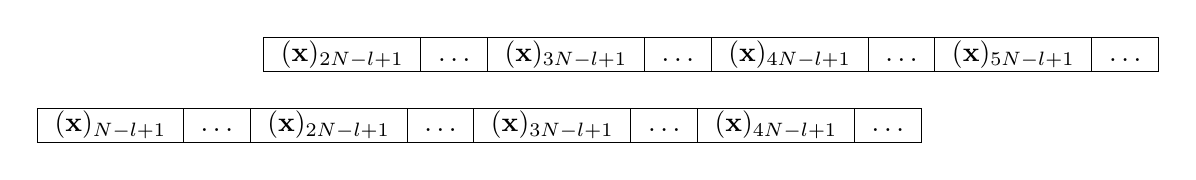
\begin{tikzpicture}
\node (species1) {
\begin{tabular}{|c|c|c|c|c|c|c|c|}\hline
    $(\vec{x})_{2N-l+1}$ & $\ldots$  & $(\vec{x})_{3N-l+1}$ & $\ldots$ & $(\vec{x})_{4N-l+1}$ & $\ldots$ & $(\vec{x})_{5N-l+1}$  & $\ldots$ \\ \hline 
    \end{tabular}
  
};
\node (species2) [below right= 0.2cm and -14.5cm of species1] {
      \begin{tabular}{|c|c|c|c|c|c|c|c|}\hline
    $(\vec{x})_{N-l+1}$ & $\ldots$  & $(\vec{x})_{2N-l+1}$ & $\ldots$ & $(\vec{x})_{3N-l+1}$ & $\ldots$ & $(\vec{x})_{4N-l+1}$  & $\ldots$ \\ \hline 
    \end{tabular}
};
\end{tikzpicture}
\caption{Example illustrating dependence, $u=L-1$}
\label{fig:ex_dep}
\end{figure}


Using this approximation, it is possible to determine the distribution of the elements  of $\vec{s}_x$: by determining the expected value ($\mu_{\omega}$) and the variance $\sigma_{\omega}^2$ for each element of $\vec{s}_x$, the distribution is completely specified.

To compute the variance of each element of $(\vec{s})_x$, we first observe that the Covariance matrix $C_{sx}$ of $\vec{s}_x$ contains the variance of each element  on the diagonal.

as $\vec{s}_x = \mat{F}\vec{\hat{r}}_x$ 

Using the Neyman Pearson Test statistic, we obtain that our threshold $\gamma_{\omega}$ given a false alarm probability $p_{fa}$ should be set to $Q^{-1}(p_{fa})\sigma_{\omega} + \mu_{\omega}$.

\end{document}